%%%%%%%%%%%%%%%%%%%%%%%%%%%%%%%%%%%%%%%%%%%%%%%%%%%%%%%%%%%%%%%%%%%%%%
% How to use writeLaTeX: 
%
% You edit the source code here on the left, and the preview on the
% right shows you the result within a few seconds.
%
% Bookmark this page and share the URL with your co-authors. They can
% edit at the same time!
%
% You can upload figures, bibliographies, custom classes and
% styles using the files menu.
%
%%%%%%%%%%%%%%%%%%%%%%%%%%%%%%%%%%%%%%%%%%%%%%%%%%%%%%%%%%%%%%%%%%%%%%

\documentclass[12pt]{article}

\usepackage{sbc-template}

\usepackage{graphicx,url}

\usepackage[brazilian]{babel}   
\usepackage[T1]{fontenc} % Codificação para fontes com suporte a caracteres acentuados
\usepackage[utf8]{inputenc} % Codificação UTF-8 (necessário apenas para pdflatex)
\usepackage{multicol}
\usepackage{multirow}
\usepackage{graphicx,url}
\usepackage{amsmath,amssymb,amsfonts}
\usepackage{algorithmic}
\usepackage{textcomp}
\usepackage{url}
\usepackage{enumerate}
\usepackage{multirow}
\usepackage{soul}
\usepackage{verbatim}
\usepackage[table,xcdraw]{xcolor}
\usepackage[shortlabels]{enumitem}
\usepackage{scalefnt} % pacote para diminuir fonte das tabelas
\usepackage{comment} % pacote de comentarios
\usepackage{lscape}
\usepackage{fancyhdr}
\usepackage{sbgames}
\usepackage[super]{nth}

%previne hifenização
\tolerance=1
\emergencystretch=\maxdimen
\hyphenpenalty=10000
\hbadness=10000

\sloppy


\trilha{Informe a Trilha} %Preencha com: Artes \& Design | Computação | Cultura | Saúde | Indústria | Educação | Tutoriais | MAGICA | WGP-Jogos
\local{Salvador/BA} % Exemplo: Manaus/AM
\ano{2025} % Exemplo: 2024
\edicao{XXIV} %Exemplo: XXIII

\title{Título em português \\
\medskip
\small{
    \textit{Title: Título em inglês}
}
}

\author{Nome Sobrenome\inst{1}, Nome Sobrenome\inst{2}, Nome Sobrenome\inst{1}, Nome Sobrenome\inst{3} }

\address{Instituto de Informática -- Universidade Federal Imaginária
  (UFI)\\
  Caixa Postal 99.999 -- 99.999-999 -- Cidade  -- DF -- Brasil
\nextinstitute
  Department of Computing Computação -- University of Somewhere\\
  Durham, U.K.
\nextinstitute
  Departamento de Sistemas e Computação\\
  Universidade Regional de Algum Lugar (UFAL) -- Blumenau, SC -- Brasil
  \email{\{author,author\}@inf.ufi.br, sobrenome@somewhere.ac.uk,
  nome@inf.ufal.br}
}


\begin{document} 

\maketitle

\thispagestyle{plain}

\begin{abstract}
\textbf{Introduction}: A good abstract, in addition to succinctly informing the content of a scientific article, serves to attract attention to the work. However, in recent years, many articles submitted to SBGames do not present any type of standardization of abstracts, which also hinders the review process.
\textbf{Objective:} Therefore, this year we will adopt a MANDATORY STRUCTURED ABSTRACT as a way to organize the work.
\textbf{Methodology or Steps}: The organization of this structured abstract follows an adaptation of ABNT 6028:2021, which deals with standards for the presentation of abstracts.
\textbf{Results:} Thus, it is expected that there will be an improvement in the presentation of abstracts and, consequently, in the quality of the articles. ATTENTION: In short papers, it should be changed to "Expected Results", since they mostly present research intentions and/or partial results.
\end{abstract}

\keywords{Word 1, Word 2, Word 3, Word 4, Word 5.}
     
\begin{resumo} 
  \textbf{Introdução:} Um bom resumo, além de informar sucintamente o conteúdo de um artigo científico, serve para atrair a atenção para o trabalho. Contudo, nos últimos anos, muitos artigos submetidos ao SBGames, não apresentam nenhum tipo de padronização dos resumos, o que, também dificulta o processo de revisão. 
  \textbf{Objetivo:} Portanto, neste ano adotaremos o RESUMO ESTRUTURADO OBRIGATÓRIO, como forma de organizar os trabalho. 
  \textbf{Metodologia ou Etapas}: A organização deste resumo estruturado segue uma adaptação da ABNT 6028:2021, que versa sobre normas para apresentação de resumos.
  \textbf{Resultados:} Assim espera-se que haja uma melhora na apresentação dos resumos e, consequentemente, na qualidade dos artigos. ATENÇÃO: Em trabalhos curtos, deve-se trocar para ``Resultados Esperados'', uma vez que eles apresentam na maioria das vezes, intenções de pesquisa e/ou resultados parciais.
\end{resumo}

\palavraschave{Palavra 1, Palavra 2, Palavra 3, Palavra 4, Palavra 5.}

\section{General Information}

All full papers and posters (short papers) submitted to some SBC conference,
including any supporting documents, should be written in English or in
Portuguese. The format paper should be A4 with single column, 3.5 cm for upper
margin, 2.5 cm for bottom margin and 3.0 cm for lateral margins, without
headers or footers. The main font must be Times, 12 point nominal size, with 6
points of space before each paragraph. Page numbers must be suppressed.

Full papers must respect the page limits defined by the conference.
Conferences that publish just abstracts ask for \textbf{one}-page texts.

\section{First Page} \label{sec:firstpage}

The first page must display the paper title, the name and address of the
authors, the abstract in English and ``resumo'' in Portuguese (``resumos'' are
required only for papers written in Portuguese). The title must be centered
over the whole page, in 16 point boldface font and with 12 points of space
before itself. Author names must be centered in 12 point font, bold, all of
them disposed in the same line, separated by commas and with 12 points of
space after the title. Addresses must be centered in 12 point font, also with
12 points of space after the authors' names. E-mail addresses should be
written using font Courier New, 10 point nominal size, with 6 points of space
before and 6 points of space after.

The abstract and ``resumo'' (if is the case) must be in 12 point Times font,
indented 0.8cm on both sides. The word \textbf{Abstract} and \textbf{Resumo},
should be written in boldface and must precede the text.

\section{CD-ROMs and Printed Proceedings}

In some conferences, the papers are published on CD-ROM while only the
abstract is published in the printed Proceedings. In this case, authors are
invited to prepare two final versions of the paper. One, complete, to be
published on the CD and the other, containing only the first page, with
abstract and ``resumo'' (for papers in Portuguese).

\section{Sections and Paragraphs}

Section titles must be in boldface, 13pt, flush left. There should be an extra
12 pt of space before each title. Section numbering is optional. The first
paragraph of each section should not be indented, while the first lines of
subsequent paragraphs should be indented by 1.27 cm.

\subsection{Subsections}

The subsection titles must be in boldface, 12pt, flush left.

\section{Figures and Captions}\label{sec:figs}


Figure and table captions should be centered if less than one line
(Figure~\ref{fig:exampleFig1}), otherwise justified and indented by 0.8cm on
both margins, as shown in Figure~\ref{fig:exampleFig2}. The caption font must
be Helvetica, 10 point, boldface, with 6 points of space before and after each
caption.

\begin{figure}[ht]
\centering
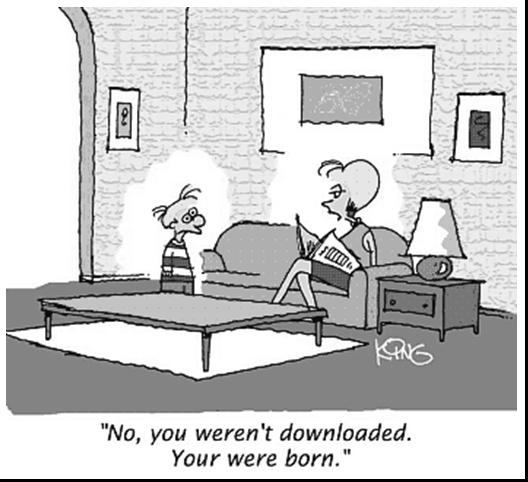
\includegraphics[width=.5\textwidth]{Figuras/fig1.jpg}
\caption{A typical figure}
\label{fig:exampleFig1}
\end{figure}

\begin{figure}[ht]
\centering
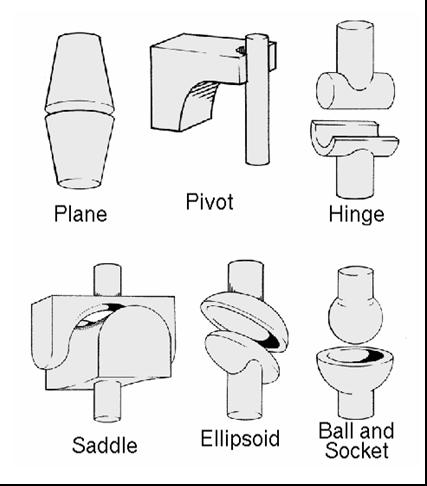
\includegraphics[width=.3\textwidth]{Figuras/fig2.jpg}
\caption{This figure is an example of a figure caption taking more than one
  line and justified considering margins mentioned in Section~\ref{sec:figs}.}
\label{fig:exampleFig2}
\end{figure}

In tables, try to avoid the use of colored or shaded backgrounds, and avoid
thick, doubled, or unnecessary framing lines. When reporting empirical data,
do not use more decimal digits than warranted by their precision and
reproducibility. Table caption must be placed before the table (see Table 1)
and the font used must also be Helvetica, 10 point, boldface, with 6 points of
space before and after each caption.

\begin{table}[ht]
\centering
\caption{Variables to be considered on the evaluation of interaction
  techniques}
\label{tab:exTable1}
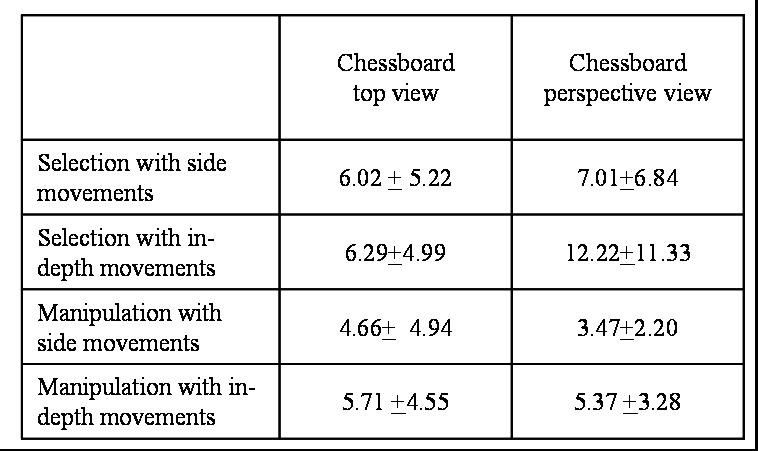
\includegraphics[width=.7\textwidth]{Tabelas/table.jpg}
\end{table}

\section{Images}

All images and illustrations should be in black-and-white, or gray tones,
excepting for the papers that will be electronically available (on CD-ROMs,
internet, etc.). The image resolution on paper should be about 600 dpi for
black-and-white images, and 150-300 dpi for grayscale images.  Do not include
images with excessive resolution, as they may take hours to print, without any
visible difference in the result. 

\section{References}

Bibliographic references must be unambiguous and uniform.  We recommend giving
the author names references in brackets, e.g. \cite{knuth:84},
\cite{boulic:91}, and \cite{smith:99}.

The references must be listed using 12 point font size, with 6 points of space
before each reference. The first line of each reference should not be
indented, while the subsequent should be indented by 0.5 cm.

\bibliographystyle{sbc}
\bibliography{Referencias/referencias}

\end{document}
